\documentclass{standalone}
\usepackage{tikz}
\usetikzlibrary{patterns, positioning}
\usepackage[sfdefault]{ClearSans} %% option 'sfdefault' activates Clear Sans as the default text font
\usepackage[T1]{fontenc}

\begin{document}
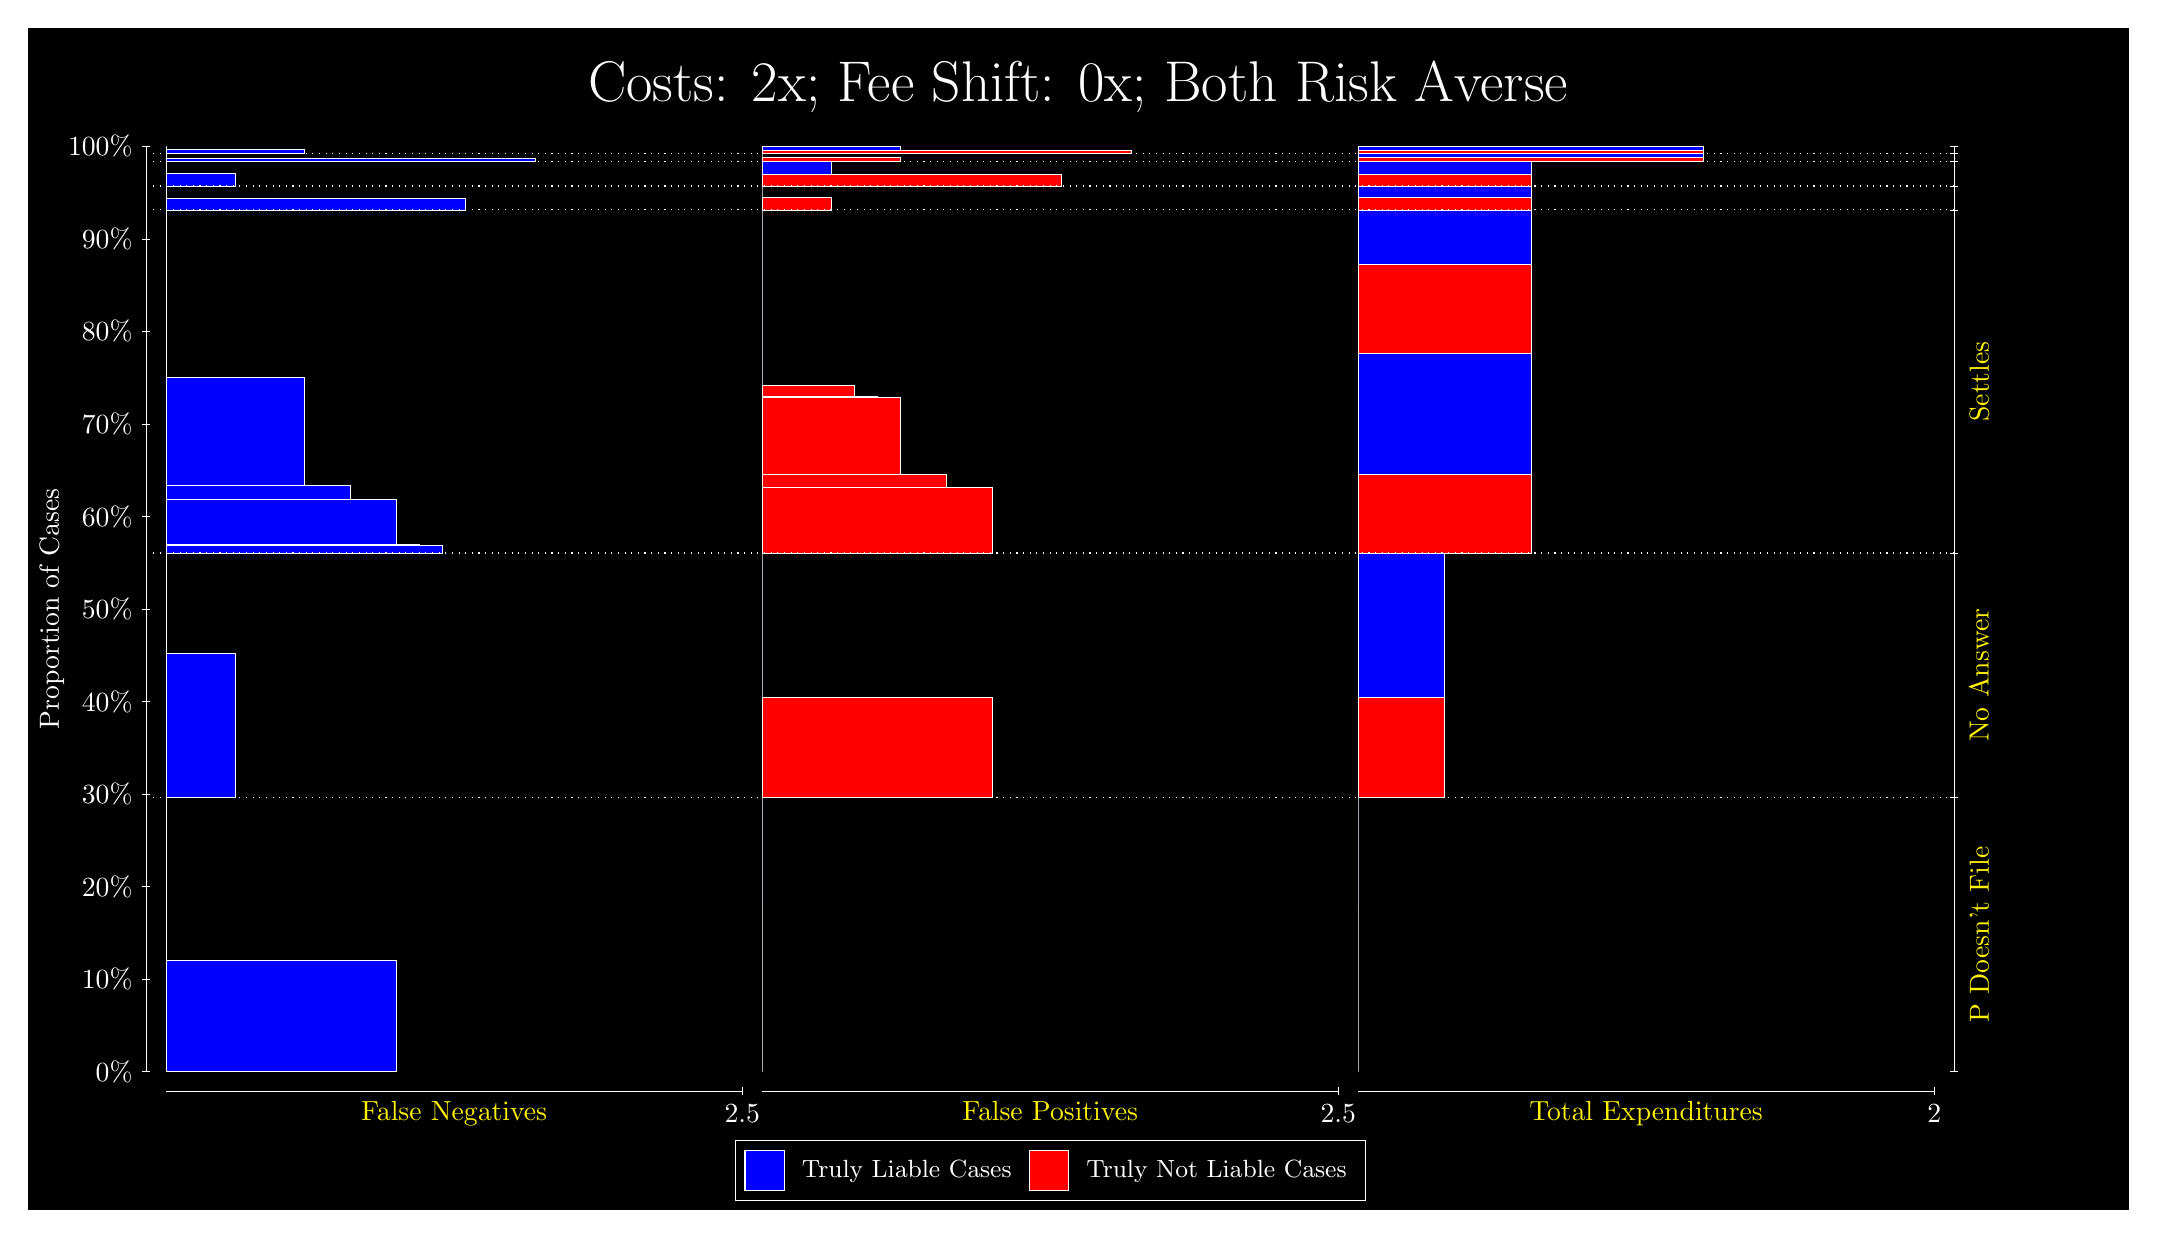
\begin{tikzpicture}
\draw[fill=black] (0,0) rectangle (26.667,15);
\draw[text=white] (0,13.5) rectangle (26.667,15) node[midway] {\huge Costs: 2x; Fee Shift: 0x; Both Risk Averse};
\draw[white, very thin] (1.5,1.75) -- (1.5,13.5);
\node[rotate=90, text=white, anchor=center] at (0.3, 7.625) {Proportion of Cases};
\draw[white, very thin] (1.45,1.75) -- (1.55,1.75);
\node[text=white, anchor=east] at (1.45, 1.75) {0\%};
\draw[white, very thin] (1.45,2.925) -- (1.55,2.925);
\node[text=white, anchor=east] at (1.45, 2.925) {10\%};
\draw[white, very thin] (1.45,4.1) -- (1.55,4.1);
\node[text=white, anchor=east] at (1.45, 4.1) {20\%};
\draw[white, very thin] (1.45,5.275) -- (1.55,5.275);
\node[text=white, anchor=east] at (1.45, 5.275) {30\%};
\draw[white, very thin] (1.45,6.45) -- (1.55,6.45);
\node[text=white, anchor=east] at (1.45, 6.45) {40\%};
\draw[white, very thin] (1.45,7.625) -- (1.55,7.625);
\node[text=white, anchor=east] at (1.45, 7.625) {50\%};
\draw[white, very thin] (1.45,8.8) -- (1.55,8.8);
\node[text=white, anchor=east] at (1.45, 8.8) {60\%};
\draw[white, very thin] (1.45,9.975) -- (1.55,9.975);
\node[text=white, anchor=east] at (1.45, 9.975) {70\%};
\draw[white, very thin] (1.45,11.15) -- (1.55,11.15);
\node[text=white, anchor=east] at (1.45, 11.15) {80\%};
\draw[white, very thin] (1.45,12.325) -- (1.55,12.325);
\node[text=white, anchor=east] at (1.45, 12.325) {90\%};
\draw[white, very thin] (1.45,13.5) -- (1.55,13.5);
\node[text=white, anchor=east] at (1.45, 13.5) {100\%};

\draw[white, very thin] (24.457,1.75) -- (24.457,13.5);
\draw[white, very thin] (24.407,1.75) -- (24.507,1.75);
\node[anchor=west] at (24.407, 1.75) {};
\draw[white, very thin] (24.407,5.2325) -- (24.507,5.2325);
\node[anchor=west] at (24.407, 5.2325) {};
\draw[white, very thin] (24.407,8.3356) -- (24.507,8.3356);
\node[anchor=west] at (24.407, 8.3356) {};
\draw[white, very thin] (24.407,12.693) -- (24.507,12.693);
\node[anchor=west] at (24.407, 12.693) {};
\draw[white, very thin] (24.407,12.996) -- (24.507,12.996);
\node[anchor=west] at (24.407, 12.996) {};
\draw[white, very thin] (24.407,13.304) -- (24.507,13.304);
\node[anchor=west] at (24.407, 13.304) {};
\draw[white, very thin] (24.407,13.406) -- (24.507,13.406);
\node[anchor=west] at (24.407, 13.406) {};
\draw[white, very thin] (24.407,13.5) -- (24.507,13.5);
\node[anchor=west] at (24.407, 13.5) {};

\draw[white, very thin, fill=blue] (1.75,1.75) rectangle (4.6775,3.1688);
\draw[white, very thin, fill=red] (1.75,3.1688) rectangle (1.75,5.2325);
\draw[white, very thin, fill=blue] (1.75,5.2325) rectangle (2.6283,7.0661);
\draw[white, very thin, fill=red] (1.75,7.0661) rectangle (1.75,8.3356);
\draw[white, very thin, fill=blue] (1.75,8.3356) rectangle (5.2631,8.4376);
\draw[white, very thin, fill=blue] (1.75,8.4376) rectangle (4.9703,8.4433);
\draw[white, very thin, fill=blue] (1.75,8.4433) rectangle (4.6775,9.0238);
\draw[white, very thin, fill=blue] (1.75,9.0238) rectangle (4.092,9.1907);
\draw[white, very thin, fill=blue] (1.75,9.1907) rectangle (3.5065,10.561);
\draw[white, very thin, fill=red] (1.75,10.561) rectangle (1.75,12.693);
\draw[white, very thin, fill=blue] (1.75,12.693) rectangle (5.5558,12.835);
\draw[white, very thin, fill=red] (1.75,12.835) rectangle (1.75,12.996);
\draw[white, very thin, fill=blue] (1.75,12.996) rectangle (2.6283,13.154);
\draw[white, very thin, fill=red] (1.75,13.154) rectangle (1.75,13.304);
\draw[white, very thin, fill=blue] (1.75,13.304) rectangle (6.4341,13.348);
\draw[white, very thin, fill=red] (1.75,13.348) rectangle (1.75,13.406);
\draw[white, very thin, fill=blue] (1.75,13.406) rectangle (3.5065,13.458);
\draw[white, very thin, fill=red] (1.75,13.458) rectangle (1.75,13.5);
\draw[white, very thin, fill=red] (9.3189,1.75) rectangle (9.3189,3.8137);
\draw[white, very thin, fill=blue] (9.3189,3.8137) rectangle (9.3189,5.2325);
\draw[white, very thin, fill=red] (9.3189,5.2325) rectangle (12.246,6.502);
\draw[white, very thin, fill=blue] (9.3189,6.502) rectangle (9.3189,8.3356);
\draw[white, very thin, fill=red] (9.3189,8.3356) rectangle (12.246,9.1641);
\draw[white, very thin, fill=red] (9.3189,9.1641) rectangle (11.661,9.3382);
\draw[white, very thin, fill=red] (9.3189,9.3382) rectangle (11.075,10.314);
\draw[white, very thin, fill=red] (9.3189,10.314) rectangle (10.783,10.321);
\draw[white, very thin, fill=red] (9.3189,10.321) rectangle (10.49,10.468);
\draw[white, very thin, fill=blue] (9.3189,10.468) rectangle (9.3189,12.693);
\draw[white, very thin, fill=red] (9.3189,12.693) rectangle (10.197,12.854);
\draw[white, very thin, fill=blue] (9.3189,12.854) rectangle (9.3189,12.996);
\draw[white, very thin, fill=red] (9.3189,12.996) rectangle (13.125,13.145);
\draw[white, very thin, fill=blue] (9.3189,13.145) rectangle (10.197,13.304);
\draw[white, very thin, fill=red] (9.3189,13.304) rectangle (11.075,13.361);
\draw[white, very thin, fill=blue] (9.3189,13.361) rectangle (9.3189,13.406);
\draw[white, very thin, fill=red] (9.3189,13.406) rectangle (14.003,13.448);
\draw[white, very thin, fill=blue] (9.3189,13.448) rectangle (11.075,13.5);
\draw[white, very thin, fill=red] (16.888,1.75) rectangle (16.888,3.8137);
\draw[white, very thin, fill=blue] (16.888,3.8137) rectangle (16.888,5.2325);
\draw[white, very thin, fill=red] (16.888,5.2325) rectangle (17.986,6.502);
\draw[white, very thin, fill=blue] (16.888,6.502) rectangle (17.986,8.3356);
\draw[white, very thin, fill=red] (16.888,8.3356) rectangle (19.083,9.3382);
\draw[white, very thin, fill=blue] (16.888,9.3382) rectangle (19.083,10.875);
\draw[white, very thin, fill=red] (16.888,10.875) rectangle (19.083,12.005);
\draw[white, very thin, fill=blue] (16.888,12.005) rectangle (19.083,12.693);
\draw[white, very thin, fill=red] (16.888,12.693) rectangle (19.083,12.854);
\draw[white, very thin, fill=blue] (16.888,12.854) rectangle (19.083,12.996);
\draw[white, very thin, fill=red] (16.888,12.996) rectangle (19.083,13.145);
\draw[white, very thin, fill=blue] (16.888,13.145) rectangle (19.083,13.304);
\draw[white, very thin, fill=red] (16.888,13.304) rectangle (21.279,13.361);
\draw[white, very thin, fill=blue] (16.888,13.361) rectangle (21.279,13.406);
\draw[white, very thin, fill=red] (16.888,13.406) rectangle (21.279,13.448);
\draw[white, very thin, fill=blue] (16.888,13.448) rectangle (21.279,13.5);
\draw[white, dotted] (1.5,5.2325) -- (24.457,5.2325);
\draw[white, dotted] (1.5,8.3356) -- (24.457,8.3356);
\draw[white, dotted] (1.5,12.693) -- (24.457,12.693);
\draw[white, dotted] (1.5,12.996) -- (24.457,12.996);
\draw[white, dotted] (1.5,13.304) -- (24.457,13.304);
\draw[white, dotted] (1.5,13.406) -- (24.457,13.406);
\draw[white, very thin] (1.75,1.5) -- (9.0689,1.5);
\node[text=yellow, anchor=north] at (5.4094, 1.5) {False Negatives};
\draw[white, very thin] (9.0689,1.45) -- (9.0689,1.55);
\node[text=white, anchor=north] at (9.0689, 1.45) {2.5};

\draw[white, very thin] (9.3189,1.5) -- (16.638,1.5);
\node[text=yellow, anchor=north] at (12.978, 1.5) {False Positives};
\draw[white, very thin] (16.638,1.45) -- (16.638,1.55);
\node[text=white, anchor=north] at (16.638, 1.45) {2.5};

\draw[white, very thin] (16.888,1.5) -- (24.207,1.5);
\node[text=yellow, anchor=north] at (20.547, 1.5) {Total Expenditures};
\draw[white, very thin] (24.207,1.45) -- (24.207,1.55);
\node[text=white, anchor=north] at (24.207, 1.45) {2};

\node[text=yellow, centered, rotate=90] at (24.777, 3.4912) {P Doesn't File};
\node[text=yellow, centered, rotate=90] at (24.777, 6.7841) {No Answer};
\node[text=yellow, centered, rotate=90] at (24.777, 10.514) {Settles};





\draw (12.978300999999998,1.5) node[draw=none] (baseCoordinate) {};
\begin{scope}[align=center]
        \matrix[scale=0.5, draw=white, below=0.5cm of baseCoordinate, nodes={draw}, column sep=0.1cm]{
            \node[rectangle, draw, minimum width=0.5cm, minimum height=0.5cm, fill=blue] {}; &
            \node[draw=none, font=\small, text=white] (B) {Truly Liable Cases}; &
            \node[rectangle, draw, minimum width=0.5cm, minimum height=0.5cm, fill=red] {}; &
            \node[draw=none, font=\small, text=white] (B) {Truly Not Liable Cases}; \\
            };
\end{scope}

\end{tikzpicture}
\end{document}